\section{Моделирование движения пассивного космического аппарата цилиндрической формы и активного космического аппарата}
\label{SEC:2SPH_MSM}

Будем рассматривать управляемое движение пассивного космического аппарата цилиндрической формы, который заменим на три заряженные сферы и будем моделировать его движение по методу многих сфер, и активного космического аппарата, движение которого будем моделировать как движение внешней сферы по методу многих сфер (рис. \ref{ris:2sph_msm}).

\begin{figure}[H]
	\center{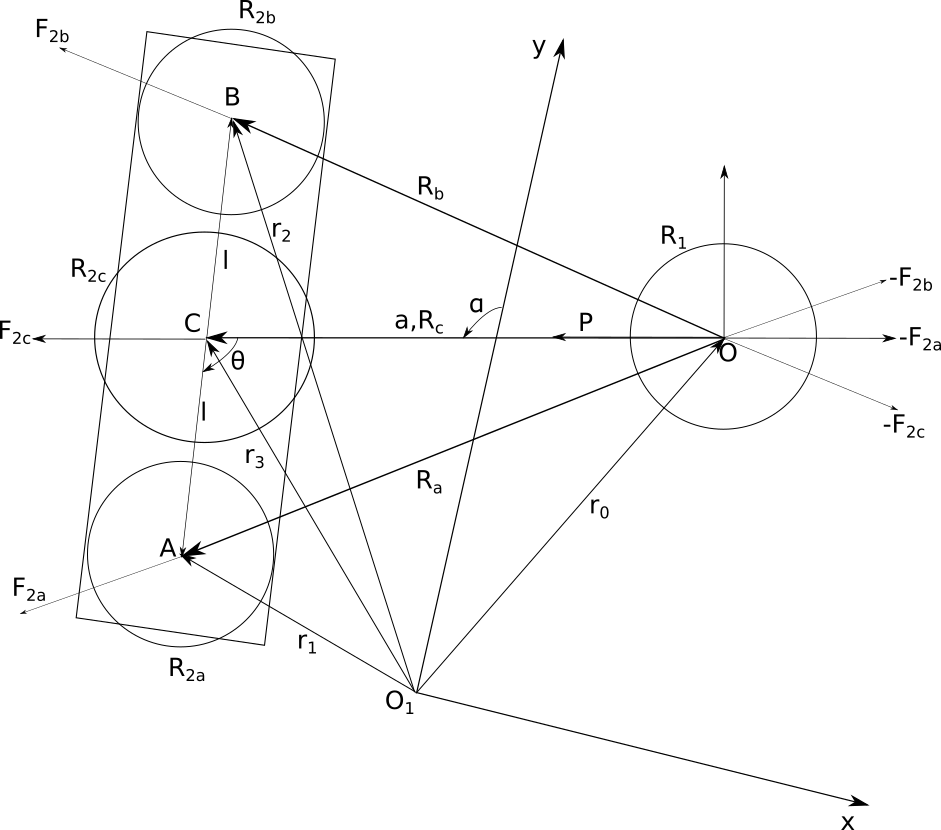
\includegraphics[scale=0.6]{2sph_msm.png}}
	\caption{Движение пассивного КА и активного КА по методу многих сфер}
	\label{ris:2sph_msm}
\end{figure}

Опишем положения сфер радиус-векторами $\vec{r}_0$, $\vec{r}_1$, $\vec{r}_2$ и $\vec{r}_3$:
\begin{equation}
\label{eq:2sph_msm_r0}
	\vec{r}_0 = 
	\begin{pmatrix}
		x\\
		y
	\end{pmatrix},
\end{equation}
\begin{equation}
\label{eq:2sph_msm_r3}
	\vec{r}_3 = \vec{r}_0 + \vec{A},
\end{equation}
где $A$ – вектор между материальными точками:
\begin{equation}
\label{eq:2sph_msm_A}
	\vec{A} = 
	\begin{pmatrix}
		- a \sin \alpha \\
		a \cos \alpha
	\end{pmatrix},
\end{equation}
где $a$ – расстояние между аппаратами, $\alpha$ – угол между вектором $A$ и осью $OY$.
\begin{equation}
\label{eq:2sph_msm_r1}
	\vec{r}_1 = \vec{r}_3 - \vec{L},
\end{equation}
\begin{equation}
\label{eq:2sph_msm_r2}
	\vec{r}_2 = \vec{r}_3 + \vec{L},
\end{equation}
где $\vec{L}$ – расстояние между сферами $C$ и $B$, $-\vec{L}$ – расстояние между сферами $A$ и $C$:
\begin{equation}
\label{eq:2sph_msm_L}
	\vec{L}_2 = 
	\begin{pmatrix}
		-l \sin(\alpha - \theta)\\
		l \cos(\alpha - \theta)
	\end{pmatrix}.
\end{equation}

Скорости центров масс тел:
\begin{equation}
\label{eq:2sph_msm_v0}
	\vec{v}_0 = \frac{d \vec{r}_0}{dt},
\end{equation}
\begin{equation}
\label{eq:2sph_msm_v1}
	\vec{v}_1 = \frac{d \vec{r}_3}{dt}.
\end{equation}

Обратная матрица емкостей для этого случая будет аналогична $[C_m]^{-1}$ (\ref{eq:3sph_cm}):
\begin{equation}
\label{eq:2sph_msm_cm}
	[C_m]^{-1} = 
	\begin{pmatrix}
		1/R_1	&	1/r_a	&	1/r_b	&	1/r_c\\
		1/r_a	&	1/R_{2a}	&	1/l		&	1/2l\\
		1/r_b	&	1/l		&	1/R_{2b}	&	1/l\\
		1/r_c	&	1/2l		&	1/l		&	1/R_{2c}
	\end{pmatrix},
\end{equation}
где $R_1$ – радиус внешней сферы, $R_{2a}$ – радиус сферы $A$ тела $2$, $R_{2b}$ – радиус сферы $B$ тела $2$, $R_{2c}$ – радиус сферы $C$ тела $2$, $l$ – расстояние между центрами соседних сфер (сферы $A$ и сферы $B$, сферы $B$ и сферы $C$),

\noindent $r_a = \norm{\vec{R}_a}$ – расстояние между центром внешней сферы и центром сферы $A$ тела $2$, $r_b = \norm{\vec{R}_b}$ – расстояние между центром внешней сферы и центром сферы $B$ тела $2$, $r_c = \norm{\vec{R}_c}$ – расстояние между центром внешней сферы и центром сферы $C$ тела $2$.

Имея (\ref{eq:2sph_msm_r0}) - (\ref{eq:2sph_msm_L}) запишем вектора $\vec{R_a}$, $\vec{R_b}$, $\vec{R_c}$:
\begin{equation}
\label{eq:2sph_msm_Ra}
	\vec{R}_a = \vec{r}_1 - \vec{r}_0,
\end{equation}
\begin{equation}
\label{eq:2sph_msm_Rb}
	\vec{R}_b = \vec{r}_2 - \vec{r}_0,
\end{equation}
\begin{equation}
\label{eq:2sph_msm_Rc}
	\vec{R}_c = \vec{r}_3 - \vec{r}_0.
\end{equation}

Далее получим обратную матрицу к матрице $[C_m]^{-1}$ (\ref{eq:2sph_msm_cm}), чем решим уравнение (\ref{eq:voltage_matr}) и получим заряды сфер аналогично разделу \ref{SEC:3SPH} (\ref{eq:3sph_q_eq}).

Запишем кинетическую энергию системы в инерциальной системе отсчета $O_1XY$:
\begin{equation}
\label{eq:2sph_msm_T}
	T = m_0 \frac{\norm{\vec{v}_0}^2}{2} + m_1 \frac{\norm{\vec{v}_1}^2}{2} + \frac{J\left(\frac{d\theta}{dt}\right)^2}{2},
\end{equation}
где $m_0$ – масса активного аппарата, $m_1$ – масса пассивного аппарата, $J$ – момент инерции пассивного аппарата.

Обобщенными координаты:
\begin{equation}
\label{eq:2sph_msm_qj}
	\begin{pmatrix}
		q_x \\
		q_y \\
		q_a \\
		q_\alpha \\
		q_\theta
	\end{pmatrix} 
	=
	\begin{pmatrix}
		x \\
		y \\
		a \\
		\alpha \\
		\theta
	\end{pmatrix}.
\end{equation}

Обобщенные силы будут иметь вид:
\begin{equation}
\label{eq:2sph_msm_Q}
	Q_j = \frac{\partial r_0}{\partial q_j} \cdot F_0 + \frac{\partial r_1}{\partial q_j} \cdot F_1 +\frac{\partial r_2}{\partial q_j} \cdot F_2 +\frac{\partial r_3}{\partial q_j} \cdot F_3,
\end{equation}
где $q_j$ – обобщенные координаты, $F_1$ – сила кулоновского взаимодействия для сферы $A$, $F_2$ – сила кулоновского взаимодействия для сферы $B$, $F_3$ – сила кулоновского взаимодействия для сферы $C$:
\begin{equation}
\label{eq:2sph_msm_f1}
	\vec{F}_1 = -\frac{k_c q_1 q_{2a}}{r_a^3}\vec{R}_a,
\end{equation}
\begin{equation}
\label{eq:2sph_msm_f2}
	\vec{F}_2 = -\frac{k_c q_1 q_{2b}}{r_b^3}\vec{R}_b,
\end{equation}
\begin{equation}
\label{eq:2sph_msm_f3}
	\vec{F}_3 = -\frac{k_c q_1 q_{2c}}{r_c^3}\vec{R}_c,
\end{equation}
$F_0$ – cила, действующая на активный аппарат:
\begin{equation}
\label{eq:2sph_msm_f0_u}
	\vec{F}_0 = \vec{P} - (\vec{F}_1 + \vec{F}_2 + \vec{F}_3) + \vec{U},
\end{equation}
где $U$ – управляющая тяга (\ref{eq:2sph_u_full}) из раздела \ref{SEC:2SPH}.

Подставив (\ref{eq:2sph_msm_T}) и (\ref{eq:2sph_msm_Q}) в уравнение Лагранжа второго рода (\ref{eq:3sph_lag}) и численно решив получившуюся систему найдем зависимости $x$, $y$, $a$, $\alpha$, $\theta$ от времени.
Зададим параметры системы $m_0 = 200$кг, $m_1=1000$кг, $p=0.2$H, $n=8.3 * 10^{-3}$, $\phi = 20000$В, $R_1 = 0.5$м, $R_{2a} = R_{2c} = 0.59$м, $R_{2b} = 0.65$м, $l = 1.5$м, $d = 15$м, $J = 1000$кг$\cdot$м${}^2$ и параметры управления $k_\alpha = -5$,$k_{\alpha t} = -2$,$k_x = 0.1$,$k_{x t} = 0.1$.
Начальные условия:
\begin{equation}
	\begin{cases}
		x(0) = 0, \\
		y(0) = 0, \\
		a(0) = 5.4, \\
		\alpha(0) = 0,\\
		\theta(0) = 0.4,\\
		x'(0) = 0, \\
		y'(0) = 0, \\
		a'(0) = 0, \\
		\alpha'(0) = 0.01\\
		\theta'(0) = 0.
	\end{cases}
\end{equation}

Решение изображено на рисунках \ref{ris:2sph_msm_a_no_u} - \ref{ris:2sph_msm_theta_no_u}.

\begin{figure}[H]
	\center{\includegraphics[scale=0.7]{2sph_msm_no_u_a.png}}
	\caption{Зависимость координаты $a$ от времени $t$ для заданных параметров}
	\label{ris:2sph_msm_a_no_u}
\end{figure}
\begin{figure}[H]
	\center{\includegraphics[scale=0.7]{2sph_msm_no_u_alpha.png}}
	\caption{Зависимость координаты $\alpha$ от времени $t$ для заданных параметров}
	\label{ris:2sph_msm_alpha_no_u}
\end{figure} 
\begin{figure}[H]
	\center{\includegraphics[scale=0.7]{2sph_msm_no_u_x.png}}
	\caption{Зависимость координаты $x$ от времени $t$ для заданных параметров}
	\label{ris:2sph_msm_x_no_u}
\end{figure} 
\begin{figure}[H]
	\center{\includegraphics[scale=0.7]{2sph_msm_no_u_y.png}}
	\caption{Зависимость координаты $y$ от времени $t$ для заданных параметров}
	\label{ris:2sph_msm_y_no_u}
\end{figure} 
\begin{figure}[H]
	\center{\includegraphics[scale=0.7]{2sph_msm_no_u_theta.png}}
	\caption{Зависимость координаты $\theta$ от времени $t$ для заданных параметров}
	\label{ris:2sph_msm_theta_no_u}
\end{figure}

Как видно из рисунков \ref{ris:2sph_msm_a_no_u} - \ref{ris:2sph_msm_y_no_u} характер движения не поменялся в сравнении с вычислениями из раздела \ref{SEC:2SPH}.
Но по рисунку \ref{ris:2sph_msm_theta_no_u} видно, что пассивный аппарат закручивается вокруг центра масс.
При сопоставимом расстоянии между аппаратами и размерами пассивного аппарата это может вызывать столкновение и короткое замыкание.
Для предотвращения закручивания используем дополнительное управление, предложенное Шаубом в \cite{3sph}.

Добавим:
\begin{equation}
\label{eq:2sph_msm_f}
	f = - k_\theta \frac{d\theta}{dt}
\end{equation}
к обобщенной силе $Q_\theta$.

Результаты численного моделирования для движения с управлением по $\theta$ при $k_\theta = 0.1$ представлены на рисунках \ref{ris:2sph_msm_a_full_u} - \ref{ris:2sph_msm_theta_full_u}.

\begin{figure}[H]
	\center{\includegraphics[scale=0.7]{2sph_msm_full_u_a.png}}
	\caption{Зависимость координаты $a$ от времени $t$ для заданных параметров с управлением по $\theta$}
	\label{ris:2sph_msm_a_full_u}
\end{figure}
\begin{figure}[H]
	\center{\includegraphics[scale=0.7]{2sph_msm_full_u_alpha.png}}
	\caption{Зависимость координаты $\alpha$ от времени $t$ для заданных параметров с управлением по $\theta$}
	\label{ris:2sph_msm_alpha_full_u}
\end{figure} 
\begin{figure}[H]
	\center{\includegraphics[scale=0.7]{2sph_msm_full_u_x.png}}
	\caption{Зависимость координаты $x$ от времени $t$ для заданных параметров с управлением по $\theta$}
	\label{ris:2sph_msm_x_full_u}
\end{figure} 
\begin{figure}[H]
	\center{\includegraphics[scale=0.7]{2sph_msm_full_u_y.png}}
	\caption{Зависимость координаты $y$ от времени $t$ для заданных параметров с управлением по $\theta$}
	\label{ris:2sph_msm_y_full_u}
\end{figure} 
\begin{figure}[H]
	\center{\includegraphics[scale=0.7]{2sph_msm_full_u_theta.png}}
	\caption{Зависимость координаты $\theta$ от времени $t$ для заданных параметров с управлением по $\theta$}
	\label{ris:2sph_msm_theta_full_u}
\end{figure}

Таким образом, как видно из рисунка \ref{ris:2sph_msm_theta_full_u}, управляющая функция (\ref{eq:2sph_msm_f}) позволяет остановить раскручивание пассивного аппарата вокруг центра масс и при этом, как видно из рисунков \ref{ris:2sph_msm_a_full_u} - \ref{ris:2sph_msm_y_full_u} не влияет на характер движения аппаратов.